\chapter{Technical Fundamentals}
Not only the medical background covered in the previous chapter, but also knowledge of the technology of mechanical heart support technologies, such as ventricular assist devices is essential for this work.
Since the main part of this thesis addresses the implementation of flow control algorithms for a left ventricular assist device, the basics of control theory and a introduction on iterative learning control will be presented here as well.

\section{Ventricular Assist Devices}
Despite the fact that heart transplantation (HTx) still is the gold standard for treatment of patients with terminal heart failure \cite{VAD2} ventricular assist devices (VADs), as a kind of mechanical circulatory support (MCS) technology, are becoming more and more important in treating patients with CVDs. There are two reasons for this. On the one hand, CVDs are gaining in importance due to demographic change. On the other hand, there is an increasing shortage of donor organs. \cite{VAD7}

\subsection{Technology}
Since the first artificial blood-pump has been implanted in 1963 \cite{VAD9} technology of VADs has improved significantly.
\\The general aim of ventricular assist devices is to provide mechanical support in pumping blood through the human body with the heart remaining inside the patients body. Assistance can either be implemented to support the heart in a counter pulsation approach, working synchronous to the heart cycle, or as an asynchronous support. Despite there being several types of VADs, all of them are working according to the same principle. Blood is taken from the circulatory system through the pumps inlet and ejected at another location via the outlet of the pump.\cite{VAD1}
\\VADs are differentiated by three criteria: the localization of the device inside the human body, the flow profile and the implantation strategy.
\\Regarding the localization of the assistance device there are three types of VADs. With around 93{\%} of all implemented devices the most commonly used ones are the left ventricular assist devices.\cite{VAD7} LVADs are placed inside the left ventricle, from where they are pumping blood into the aorta \cite{VAD4}. The second localization option is given by placing the device as a support for  the right ventricle. These devices are therefore called right ventricular assist devices (RVADs). RVADs are positioned such that blood is taken from the right atrium and ejected into the pulmonary artery. \cite{VAD7} In some cases RVADs in combination with the aforementioned LVADs are used to build a biventricular assist device (BVAD). This type of heart support is mainly used for more severe heart diseases with a high risk of developing right heart failure. \cite{VAD11}
\\The flow profile as the second criterion for VAD distinction is represented through pulsatile and continuous flow devices. The most commonly known type of pulsatile device is a pneumatically driven pump ventricle. \cite{VAD1}
%These kind of VAD are especially important as up to now they are the only option enabling pediatric mechanical circulatory support. \cite{VAD1}
However, according to the Interagency Registry for Mechanically Assisted Circulatory Support (INTERMACS) over 95{\%} of all implanted devices are continuous flow devices \cite{VAD8}. These, in their most commonly used form, are electrically driven rotational blood pumps. A technological difficulty with these devices is the high probability of blood damage due to small gaps and very high rotational speed. In exchange for this problematic these devices enable a dynamic adaption to the patients physiological needs by being able to quickly adjusting parameters like the motor current. The possibility of keeping track of these signal characteristics furthermore makes it possible to detect malfunctions such like misplacement of the pump. \cite{VAD1}
\\Implantation of the VADs can be performed in one of three ways: paracorporeal, intracorporeal or percutaneous \cite{VAD7}. For VAD systems which follow a paracorporeal approach, only the in- and outflow cannulas are located inside the human body. The cannulas are connecting the pump, which is located outside the body, with the ventricle and the vessels. Due to the pump being placed outside of the patients body, these systems provide the option for pediatric MCS. For most other systems this is not possible due to the device being to big to fit inside a child's body. \cite{VAD10} One example for paracorporeal systems are the aforementioned pneumatically driven pump ventricles \cite{VAD1}. As far as the other two criteria for VAD differentiation are concerned, all combinations of localization and flow control are possible \cite{VAD10}. As an example of a percutaneous device, \cite{VAD7} names the Impella 2.5, which is a rotary blood pump with continuous flow used for left ventricular assistance.

\subsection{Therapeutic objective}
Traditionally the therapeutic goals of VAD treatment can be divided into three categories: \textit{bridging to transplantation} (BTT), \textit{bridging to recovery} (BTR) and \textit{destination therapy} (DT). However in some cases also the classification into \textit{bridging to decision} (BTD) and \textit{bridging to transplantability} are mentioned as well. The decision for one of these goals is based on the type of CVD and the condition the patient is in, when receiving VAD assistance.\cite{VAD6} An overview on the relation between the INTERMACS Score, the New York Heart Association(NYHA)-classification and the patient's condition is presented in \tablename~ \ref{tab:Table1}.
\begin{table}
  \begin{tabularx}{\textwidth}{l|c|l|l}
    %\hline
    \toprule
    INTERMACS & NYHA & Patient condition & Survival time  \\
    Score & & &\\
    \midrule
    %\hline
    1 & IV & critical cardiogenic shock & hours \\
    2 & IV & increasing catecholamine demand & days \\
    3 & IV & stable under inotropics & a week \\
    4 & IV & frequent decompensation & weeks-month \\
    5 & IV & rest discomfort/ not resilient & weeks-month \\
    6 & IV & rest discomfort/ merely resilient & month \\
    7 & IIIb & merely resilient & one year survival rate: \\
     & & & 50-70\% \\
     \bottomrule
  %  \hline
  \end{tabularx}
  \caption{Relation between INTERMACS Score, NYHAc-classification, patient condition and approximate survival time based on \cite{VAD5}}
  \label{tab:Table1}
\end{table}
The INTERMACS Score, which is based on data from patients which have received VAD treatment, links the need for a VAD and the appropriate time frame in which the devices needs to be implanted. It is of high importance in the decision of the therapeutic objective for VAD treatment. \cite{VAD7}
\\The goal of \textit{bridging to transplantation} has a big relevance with patients in NYHA-IV Stadium which are showing hemodynamical instability. Due to a heart transplantation being the desired final treatment for these patients there must be no contraindication to HTx. In case the patient does show a contraindication, such as malignant tumors or an uncontrollable sepsis, the therapeutic objective changes from BTT to DT. In order for a treatment with a VAD as destination therapy being indicated all conservative treatment options need to be exhausted. Due to the ever-growing shortage of donor organs DT as a therapeutic approach in patients with heart insufficiency will become more relevant in the future even in cases usually suited for heart transplantation. \cite{VAD7} There may occur some cases, in which at first a contraindication for HTx exists, which later on may dissolve. These indicate a therapy based on a \textit{bridging to transplantability} goal. \cite{VAD6}
\\The indication for a \textit{bridging to recovery} approach is twofold. Either the patient shows heart failure as a result of ischemia reperfusion damage or due to infectious genesis. In the first case the myocardium usually is able to recover within a few days, whereas in the second one the potential and the time necessary for recovery depends on how badly the tissue is damaged. In either scenario a weaning from the VAD is an essential part of therapy. \cite{VAD7}
\\If a patient is admitted in cardiogenic shock and medical treatment is not sufficient, \textit{bridging to decision} becomes a relevant form of therapy. By providing the patient with a VAD, a more accurate assessment of the patient's condition is possible.
Based on this, the decision on further treatment can be thought through more thoroughly. \cite{VAD6} \tablename~ \ref{tab:Table2} illustrates the proportions of different VAD types and therapeutic goals using the International Mechanically Assisted Circulatory Support (IMACS) register.
\begin{table}
  \centering
  \begin{tabular}{cc|cc}
    %\hline
    \toprule
    \multicolumn{2}{c|}{VAD type} &
    \multicolumn{2}{c}{Therapeutic objective} \\
    %\hline
    \midrule
    LVAD & 93\% & DT & 40\%\\
    BVAD & 4\% & BTD & 30\%\\
    TAH & 2\% & BTT & 29\%\\
    unknown & 0.1\% & others (BTR,...) & 1\%\\
    RVAD & 0.05\% & &\\
    %\hline
    \bottomrule
\end{tabular}
  \caption{Percentages of VAD types and thearapeutic objectives in mechanical heart supports based on \cite{VAD7}.}
  \label{tab:Table2}
\end{table}

\section{Control Theory}
Since the field of control theory is very extensive, this section will only deal with the notation and structure of a standard control loop in general. Furthermore, the basic principles of a PI controller and an iterative learning control are discussed, since these are used within pratical part of the thesis.

The basic task of control engineering is to influence a time-varying process from the outside with the goal that the process is executed in a predetermined manner. A control system is characterized in particular by the feedback of the controlled variable to the reference variable. The reference variable represents the state to be achieved.
In theory, this is represented by a control loop with the components shown in \figurename~{\ref{fig:control_loop}}.
The plant $G(s)$ transfers the actuating variable $u(t)$, as well as the influence of the the disturbance $d(t)$, to the controlled variable $y(t)$. This variable is permanently compared with the reference variable $w(t)$ by means of a feedback. Which results in the control error
\begin{equation}
  e(t) = w(t) - y(t)
 \label{eq:e_t}
\end{equation}
The controller $G_{c}(s)$ then transfers the control error to the actuating variable again. The aim of the control loop is to achieve the smallest possible control error with the greatest possible damping. Since these goals contradict each other, a trade off must always be accepted here.\cite{Reg_17}
\\However, there are some general requirements for the closed control loop, which have to be fulfilled. The first of which states that the closed loop needs to be stable. This is the case when the control loop responds to a finite excitation with a finite output signal. The second one is the requirement for disturbance rejection, stating that the controlled variable needs to follow the reference variable asymptotically, so that
\begin{equation}
    \lim\limits_{t \rightarrow \infty}{e(t)} = 0
 \label{eq:lim_e}
\end{equation}

\begin{figure}
  \centering
  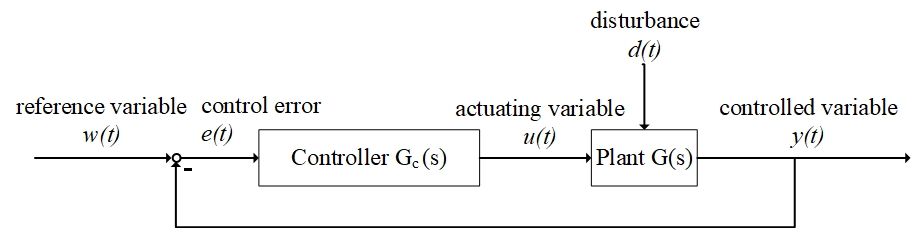
\includegraphics[width=0.9\textwidth]{images/control_loop.jpg}
  \caption{General structure of a control loop}
  \label{fig:control_loop}
\end{figure}
\subsection{PI Controller}
\subsubsection{Chien Hrones Reswick}
\subsection{Iterative Learning Control}
